
\chapter{Metodyka pracy oraz przygotowanie infrastruktury informatycznej}

\section{Wstęp}
Projekt powstawał w metodyce DevOps. Takie podejście pozwoliło na szybsze dostarczenie finalnego produktu. Wysoki poziom kooperacji wynikający z metodki DevOps pozwolił na zmniejszenie kosztów dostarczenia produktu oraz znaczne zwiększenie jego spójności. Potrzebna jest jednak mocno rozwinięta infrastruktura informatyczna służąca podtrzymaniu DevOps lifecycle.

\section{Pojęcia}
	\subsection{DevOps}
	DevOps~\cite{devops} to zestaw praktyk, narzędzi i filozofii kulturowej, które automatyzują i integrują procesy pomiędzy zespołami programistów oraz IT. Kładzie nacisk na wzmocnienie pozycji zespołu, komunikację i współpracę między zespołami oraz automatyzację technologii.
	Ruch DevOps rozpoczął się około 2007 roku, kiedy społeczności programistów i operatorów IT wyraziły zaniepokojenie tradycyjnym modelem rozwoju oprogramowania, w którym programiści piszący kod pracowali oddzielnie od operatorów, którzy wdrażali i wspierali kod. Termin DevOps, będący połączeniem słów \textit{development} i \textit{operations}, odzwierciedla proces integracji tych dyscyplin w jeden, ciągły proces (zob.~rysunek~\ref{rys:devops_lifecycle}).
\begin{figure}[H]
\centering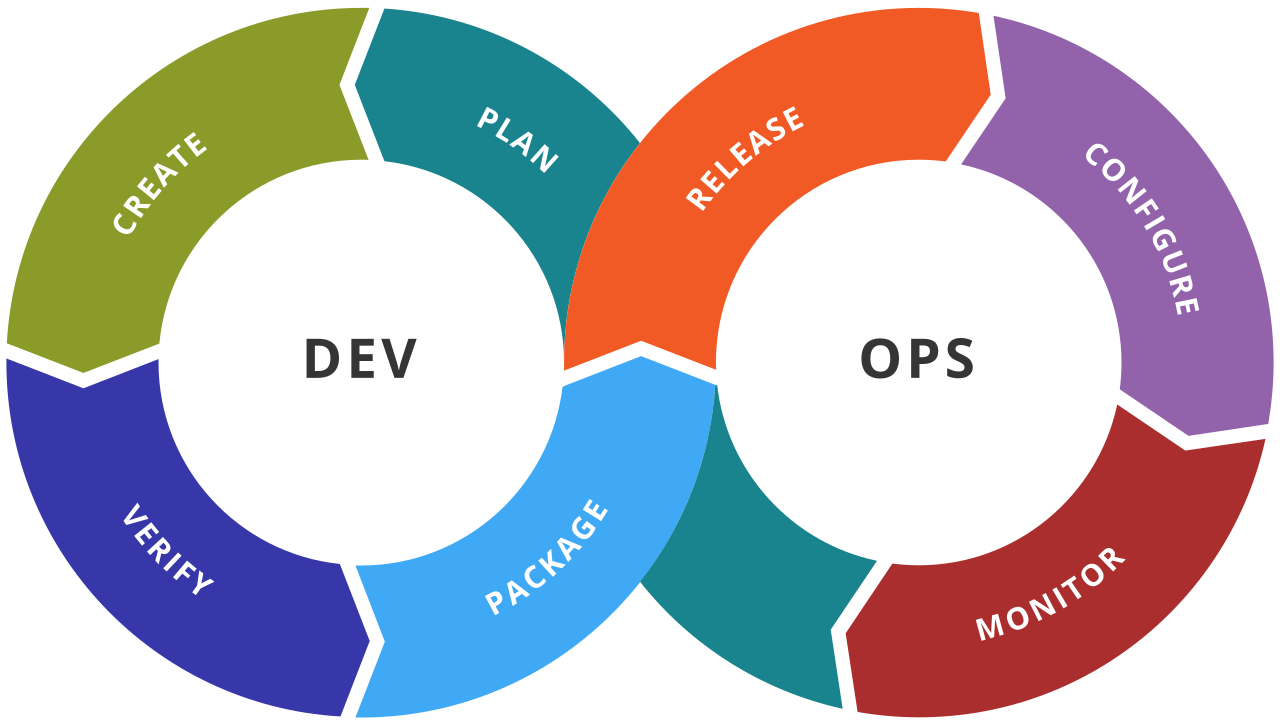
\includegraphics[width=10cm]{figures/devops_lifecycle}
\caption{Schemat DevOps lifecycle~\cite{devops_lifecycle}}\label{rys:devops_lifecycle}
\end{figure}

	\subsection{Continous Integration and Continous Deployment}
	\textit{Continous Integration and Continous Deployment} (CI/CD)~\cite{ci} to metoda częstego dostarczania aplikacji do klientów poprzez wprowadzenie automatyzacji do etapów tworzenia aplikacji. Główne pojęcia przypisane do CI/CD to ciągła integracja, ciągłe dostarczanie i ciągłe wdrażanie. CI/CD jest rozwiązaniem problemów, jakie integracja nowego kodu może powodować dla zespołów programistycznych i operacyjnych.
	W szczególności, CI/CD wprowadza ciągłą automatyzację i ciągłe monitorowanie w całym cyklu życia aplikacji, od fazy integracji i testowania po dostarczanie i wdrażanie. Łącznie, te połączone praktyki są często określane jako CI/CD i są wspierane przez zespoły programistów i operatorów pracujących razem z podejściem DevOps lub SRE (\textit{site reliability engineering}).
	
	\subsection{Kontrola wersji}
	Kontrola wersji~\cite{version_control}, znana również jako kontrola źródła, jest praktyką śledzenia i zarządzania zmianami w kodzie oprogramowania. Systemy kontroli wersji to narzędzia programowe, które pomagają zespołom programistów zarządzać zmianami w kodzie źródłowym w czasie.


\section{Narzędzia i technologie}
	\subsection{Amazon Web Services}
	\textit{Amazon Web Services} (AWS)~\cite{aws} jest spółką zależną firmy Amazon, dostarczającą platformy chmury obliczeniowej na żądanie oraz interfejsy API osobom prywatnym, firmom i rządom na zasadzie \textit{pay-as-you-go}. Te usługi internetowe w chmurze obliczeniowej zapewniają różnorodne podstawowe abstrakcyjne elementy infrastruktury technicznej oraz narzędzia i bloki do obliczeń rozproszonych. Jedną z tych usług jest \textit{Amazon Elastic Compute Cloud} (EC2), która pozwala użytkownikom mieć do dyspozycji wirtualny klaster komputerów, dostępny przez cały czas, przez Internet. Wirtualne komputery AWS emulują większość atrybutów prawdziwego komputera, w tym sprzętowe jednostki centralne (CPU) i procesory graficzne (GPU) do przetwarzania danych, pamięć lokalną/RAM, pamięć masową HDD/SSD, wybór systemów operacyjnych, sieci oraz wstępnie załadowane oprogramowanie użytkowe, takie jak serwery internetowe, bazy danych i zarządzanie relacjami z klientami (CRM).
	
	\subsection{Git}
	Git~\cite{git} to darmowe narzędzie open-source służące do kontroli wersji, zaprojektowane do obsługi wszystkiego, od małych do bardzo dużych projektów z dużą prędkością i wydajnością.	
	
	\subsection{GitHub}
	GitHub~\cite{github} jest dostawcą hostingu internetowego dla rozwoju oprogramowania i kontroli wersji przy użyciu Git. Oferuje on funkcje rozproszonej kontroli wersji i zarządzania kodem źródłowym (SCM) Git, a także własne funkcje.
	
	\subsection{Docker}
	Docker~\cite{docker} to platforma konteneryzacji typu open source. Umożliwia ona programistom pakowanie aplikacji w kontenery -- ustandaryzowane komponenty wykonywalne łączące kod źródłowy aplikacji z bibliotekami systemu operacyjnego (OS) i zależnościami wymaganymi do uruchomienia tego kodu w dowolnym środowisku. Kontenery upraszczają dostarczanie aplikacji rozproszonych i stają się coraz bardziej popularne w miarę jak organizacje przechodzą na rozwój cloud-native i hybrydowe środowiska wielochmurowe.
	
	\subsection{CircleCI}
	CircleCI~\cite{circleci} jest platformą obsługującą \textit{Continous Integration and Continous Delivery} (CI/CD), która pomaga zespołom programistycznym szybko i pewnie wypuszczać kod poprzez możliwość tworzenia \textit{pipeline} (brak odpowiednika w języku polskim) automatyzujących proces budowania, testowania i wdrażania. Pozwala to zespołom szybko się rozwijać, łatwo skalować i budować spójne produkty (zob.~rysunek~\ref{rys:circleci_diagram}).
	\begin{itemize}
	\item \textit{Pipeline} jest jednostką pracy najwyższego poziomu, obejmującą cały plik ,,.circleci/config.yml'' projektu. \textit{Pipeline} zawiera przepływy pracy (\textit{workflow}), które koordynują zadania. Mają one ustalony, liniowy cykl życia i są powiązane z konkretnym aktorem. \textit{Pipeline} uruchamia się po wprowadzeniu zmiany do projektu, który zawiera plik konfiguracyjny CircleCI, a także mogą być zaplanowane, uruchamiane ręcznie za pomocą aplikacji CircleCI lub interfejsu API.
	\end{itemize}
\begin{figure}[H]
\centering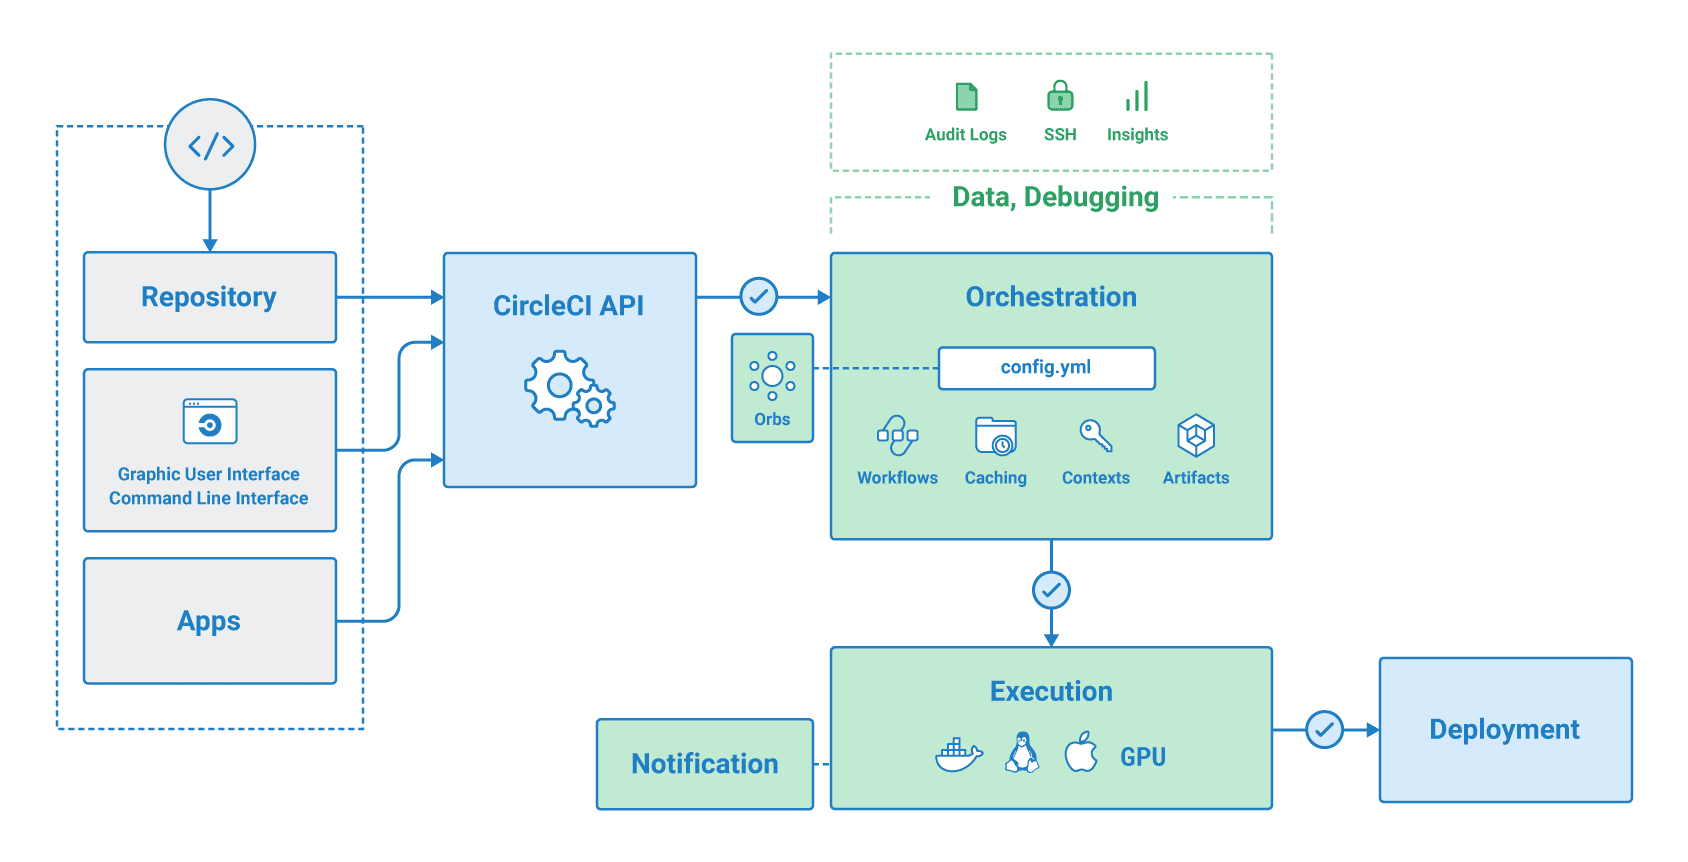
\includegraphics[width=\textwidth]{figures/circleci_schema}
\caption{Diagram przedstawiający działanie CircleCI~\cite{circleci_schema}}\label{rys:circleci_diagram}
\end{figure}

	\subsection{Secure Shell}
	\textit{Secure Shell} (SSH)~\cite{ssh} to protokół zdalnej administracji, który pozwala użytkownikom kontrolować i modyfikować zdalne serwery przez Internet. Usługa ta została stworzona jako bezpieczny zamiennik dla nieszyfrowanego protokołu Telnet i wykorzystuje techniki kryptograficzne, aby zapewnić szyfrowaną komunikację ze zdalnym serwerem. Zapewnia mechanizm uwierzytelniania zdalnego użytkownika, przesyłania danych wejściowych od klienta do hosta i przekazywania danych wyjściowych z powrotem do klienta.
	
	\subsection{tmux}
	tmux~\cite{tmux} jest multiplekserem terminali. Umożliwia tworzenie, dostęp i sterowanie wieloma terminalami z jednego ekranu. tmux może zostać odłączony od ekranu i kontynuować pracę w tle, a następnie ponownie dołączony.
	
	\subsection{shell}
	\textit{Shell}~\cite{shell} to termin UNIX dla interaktywnego interfejsu pośredniczącego między użytkownikiem a systemem operacyjnym. \textit{Shell} jest warstwą programowania, która rozumie i wykonuje polecenia wprowadzane przez użytkownika. W niektórych systemach, powłoka nazywana jest interpreterem poleceń. \textit{Shell} zwykle implikuje interfejs ze składnią poleceń.
	
	\subsection{Black}
	Black~\cite{black} jest formaterem kodu w języku Python. Wykorzystanie gotowego rozwiązania oraz zastosowanie go dla wszystkich plików  ,,.py'' standaryzuje kod co znacznie ułatwia pracę nad większym projektem.
	
	\subsection{Pylint}
	Pylint~\cite{pylint} jest narzędziem do statycznej analizy kodu w języku Python. Pylint szuka błędów programistycznych, pomaga egzekwować standardy kodowania i oferuje proste sugestie refaktoryzacji.

\section{Przygotowanie infrastruktury informatycznej}
	\subsection{Przygotowanie strony serwerowej przy pomocy platformy AWS}
	Do przygotowania strony serwerowej aplikacji wykorzystano jedną z usług platformy \textit{Amazon Web Services} jaką jest \textit{Amazon Elastic Compute Cloud} (EC2). Do przygotowania serwera strony frontendowej oraz backendowej przygotowano dwie niezależne instancje usługi EC2. Obie z przygotowanych instancji są typu \textit{t2.micro} zawierającego się w ramach pakietu \textit{AWS Free Tier}. Dzięki wyborowi tego typu instancji udało się zachować zerowy wkład pieniężny na potrzeby pracy inżynierskiej. Zasoby możliwe do wykorzystania w ramach typu \textit{t2.micro} nie są wystarczające na przypadek skomercjalizowania projektu jednak w zupełności wystarczają na potrzeby przygotowania projektu w ramach pracy inżynierskiej.
System operacyjny wykorzystany na obu instancjach EC2 to \textit{Linux Ubuntu 20.04.3 LTS} w wersji serwerowej. Zastosowanie takiej wersji systemu zmniejsza zapotrzebowanie systemu na zasoby obliczeniowe przez ograniczenie procesów systemowych (np. brak GUI) dzięki czemu większa ilość zasobów może zostać udostępniona na potrzeby zadań serwerowych. W celu zwiększenia bezpieczeństwa komunikacji, reguły połączeń przychodzących (\textit{Inbound Rules}) oraz reguły połączeń wychodzących (\textit{Outbound Rules}) zostały skonfiguorwane tak, aby jak najbardziej uszczegółowić typy możliwych połączeń z instancjami.
	
	\subsection{Przygotowanie CI/CD Pipeline przy pomocy platformy CircleCI}
	Do przygotowania \textit{CI/CD pipeline} wykorzystano platformę CircleCI. Cały proces przygotowano w taki sposób aby \textit{pipeline} uruchamiany został w momencie wprowadzenia zmian w repozytorium. Zadanie \textit{job} budowania (\textit{build}) i testowania (\textit{test}) uruchamiane jest dla każdych zmian wprowadzonych w zdalnym repozytorium. Zadanie wdrażania (\textit{deployment}) uruchamiane jest tylko i wyłącznie, jeśli zmiany zostały wprowadzone w ramach gałęzi Git (\textit{branch}) \textit{main} oraz jeśli zadanie budowania i testowania zakończyło się bez błędów (zob.~rysunek~\ref{rys:passed_ppl} oraz ~rysunek~\ref{rys:error_ppl}).

	
\begin{figure}[H]
\centering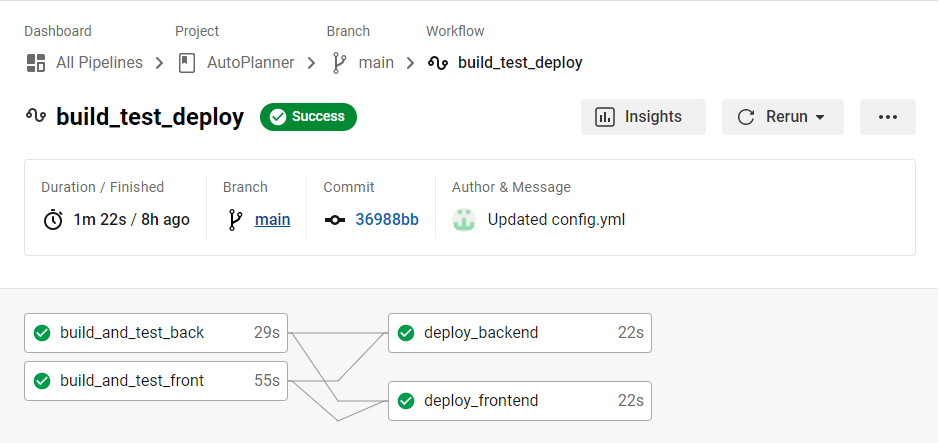
\includegraphics[width=\textwidth]{figures/ppl_flow}
\caption{Pipeline uruchomiony dla zmian wprowadzonych w gałęzi Git \textit{main}.}\label{rys:passed_ppl}
\end{figure}

\begin{figure}[H]
\centering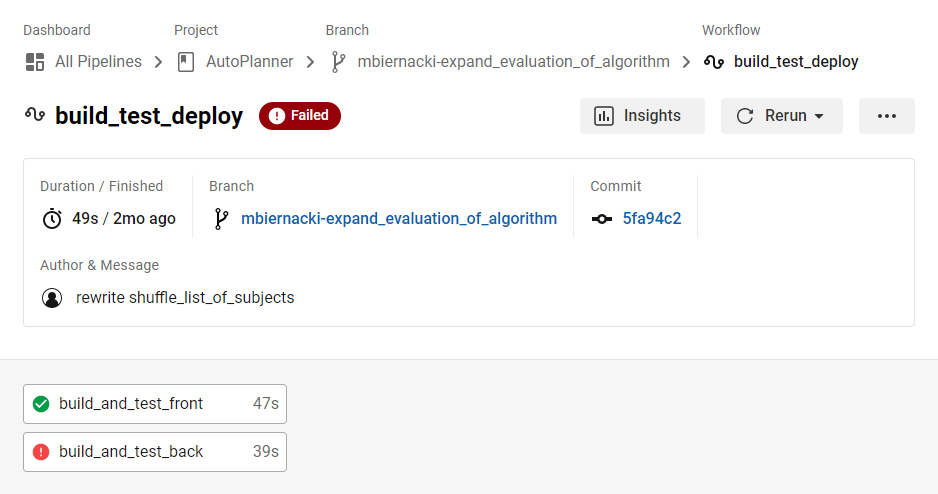
\includegraphics[width=\textwidth]{figures/ppl_flow_fail}
\caption{Pipeline, w którym wystąpiły błędy. Uruchomiony dla zmian wprowadzonych w gałęzi Git innej niż \textit{main}.}\label{rys:error_ppl}
\end{figure}

	Każdy przepływ pracy składa się z zadań, na które składają się jeszcze mniejsze kroki, podczas których wywoływane mogą być polecenia interfejsu \textit{shell}, wykonywane w kontenerach Docker stworzonych na potrzeby wykonania danego zadania. Platforma CircleCI umożliwia tworzenie własnych obrazów Docker jak i zarówno dostarcza szereg gotowych rozwiązań przygotowanych w celu ułatwienia i przyśpieszenia tworzenia \textit{pipeline} na potrzeby małych projektów. Na potrzeby projektu inżynierskiego utworzono przepływ pracy \textit{build\_test\_deploy} składający się z 4 zadań \textit{build\_and\_test\_back, build\_and\_test\_front, deploy\_frontend} oraz \textit{deploy\_backend} (zob.~listing~\ref{lst:workflow}).
	
\newpage
\begin{itemize}
	\item \textit{build\_and\_test\_back} -- podczas tego kroku budowany jest kontener Docker na bazie obrazu z przygotowanym Pythonem w wersji 3.9. Na początku tego zadania w obrębie kontenera wykonywane jest przełączenie (\textit{checkout}) na gałąź Git, której zmiany wywołały start \textit{pipeline}. Następnie wykonywany jest krok instalujący wymagania projektowe (\textit{requirements}) z pliku ,,requirements.txt''. Kolejnym krokiem jest sformatowanie plików ,,.py'' przy pomocy gotowego rozwiązania jakim jest narzędzie Black. Następny krok to sprawdzenie kodu przy pomocy Pylint. Wykorzystanie tego narzędzia zwiększa jakość publikowanego kodu oraz go standaryzuje w przypadku rozwijania oprogramowania przez wiele osób. Dwa ostatnie kroki odpowiedzialne są za uruchomienie testów jednostkowych backendu oraz algorytmu (zob.~listing~\ref{lst:test_back} oraz ~rysunek~\ref{rys:test_back}).
	\item \textit{build\_and\_test\_front} -- w tym zadaniu na początku budowany jest kontener Docker na bazie obrazu z przygotowanym Node.js w wersji 17.2.0. Następnie wykonywane jest przełączenie do gałęzi Git, której zmiany wywołały start \textit{pipeline}.  Kolejne dwa kroki odpowiedzialne są za przygotowanie środowiska tj. zaktualizowanie wersji Node.js do \textit{latest} oraz zainstalowanie dependencji projektu. W tak przygotowanym środowisku ostatnim krokiem jest uruchomienie testów jednostkowych z przygotowanego pliku (zob.~listing~\ref{lst:test_front} oraz ~rysunek~\ref{rys:test_front}).
	\item \textit{deploy\_frontend} -- w tym zadaniu głównym narzędziem jest aws-cli (\textit{AWS command line interface}). Pozwala on na obsługę instancji EC2 z poziomu interfejsu \textit{shell}. Pierwszym krokiem zadania jest przełączenie do gałęzi Git, której zmiany wywołały wystartowanie \textit{pipeline}. W nastepnym kroku ustawiany jest \textit{access\_key\_id} oraz \textit{secret\_access\_key} potrzebny do połączenia SSH. Dzięki wykorzystaniu zmiennych środowiskowych platformy CircleCI wartości te pozostają ukryte dla osób nie mających dostępu do projektu z poziomu platformy. Ostatnim jednak bardzo rozbudowanym krokiem jest połączenie z użyciem protokołu SSH i wykonanie operacji wdrożenia z poziomu instancji serwera. Po podłączeniu się do maszyny zdalnej wykonywane są takie czynności jak pobranie (\textit{pull}) najnowszych zmian ze zdalnego repozytorium, reinstalacja dependencji oraz restart serwera frontendowego. Po stronie serwera wykorzystywane jest narzędzie tmux. Dzięki otwarciu sesji w tle, możliwe jest wykonywanie innych czynności z równolegle działającym serwerem oraz utrzymanie sesji serwera po zakończeniu sesji \textit{SSH} (zob.~listing~\ref{lst:deploy_front} oraz ~rysunek~\ref{rys:deploy_front}).
	\item \textit{deploy\_backend} -- podobnie jak w zadaniu \textit{deploy\_frontend} głównym narzędziem jest aws-cli. Pierwszym krokiem zadania jest przełączenie do gałęzi Git, której zmiany wywołały wystartowanie \textit{pipeline}. W następnym kroku ustawiany jest \textit{access\_key\_id} oraz \textit{secret\_access\_key} potrzebny do połączenia SSH. Dzięki wykorzystaniu zmiennych środowiskowych platformy CircleCI wartości te pozostają ukryte dla osób nie mających dostępu do projektu z poziomu platformy. Ostatnim krokiem jest połączenie z użyciem protokołu SSH i wykonanie operacji wdrożenia z poziomu instancji serwera. Po rozpoczęciu sesji zdalnej z instancją serwera, wykonywane są takie czynności jak pobranie najnowszych zmian ze zdalnego repozytorium, reinstalacja wymagań projektowych z pliku ,,requirements.txt'' oraz restart serwera backendowego. Po stronie serwera wykorzystywane jest narzędzie tmux (zob.~listing~\ref{lst:deploy_back} oraz ~rysunek~\ref{rys:deploy_back}).
\end{itemize}
	
\newpage
	
\begin{lstlisting}[caption=Część skryptu config.yml odpowiedzialna za określenie przepływów pracy,label={lst:workflow}]
workflows:
  build_test_deploy:
    jobs:
      - build_and_test_back
      - build_and_test_front
      - deploy_frontend:
          requires:
            - build_and_test_back
            - build_and_test_front
          filters:
            branches:
              only:
                - main
      - deploy_backend:
          requires:
            - build_and_test_back
            - build_and_test_front
          filters:
            branches:
              only:
                - main
\end{lstlisting} 


	
\begin{lstlisting}[caption=Część skryptu config.yml odpowiadająca za wykonanie zadania \textit{build\_and\_test\_back},label={lst:test_back}]
build_and_test_back:
    docker:
      - image: cimg/python:3.9
    steps:
      - checkout
      - run:
          name: Install requirements
          command:
            sudo apt-get update;
            pip install --upgrade pip && pip install -r requirements.txt && pip install pylint
      - run:
          name: Format .py files
          command:
            pip install black && black $(git ls-files '*.py')
      - run:
          name: pylint
          command:
            pylint $(git ls-files '*.py')
      - run:
          name: unit_test_django
          command:
            cd Backend && python manage.py test backend_api
      - run:
          name: unit_test_algorithm
          command:
            cd Algorithm && pytest
\end{lstlisting} 
\begin{figure}[H]
\centering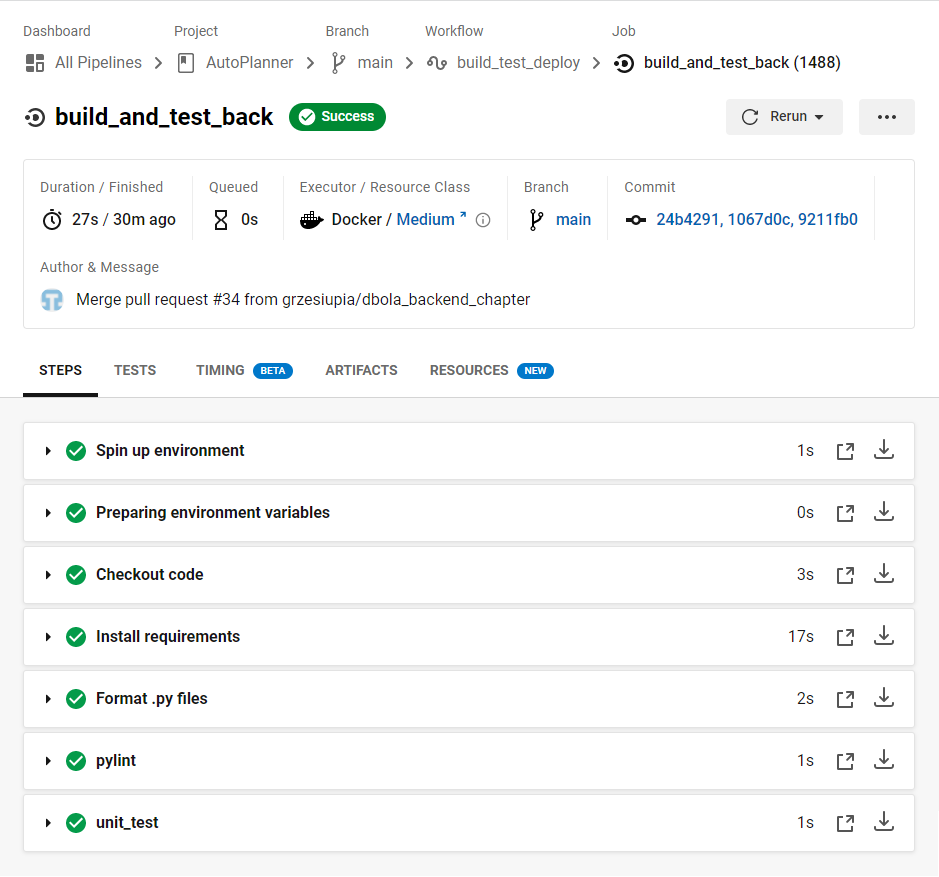
\includegraphics[width=14cm]{figures/circleci_test_back}
\caption{Przykładowy przebieg zadania \textit{build\_and\_text\_back}. Uruchomiony dla zmian wprowadzonych w gałęzi Git \textit{main}.}\label{rys:test_back}
\end{figure} 


\begin{lstlisting}[caption=Część skryptu config.yml odpowiadająca za wykonanie zadania \textit{build\_and\_test\_front},label={lst:test_front}]
build_and_test_front:
    docker:
      - image: cimg/node:17.2.0
    steps:
      - checkout
      - run:  
          name: Update node.js
          command:
            npm install node.js@latest
      - run:
          name: Install dependencies
          command:
            npm install ./Frontend
      - run:
          name: unit_tests
          command:
            cd Frontend &&
            npm run test:unit
\end{lstlisting}
\newpage
\begin{figure}[H]
\centering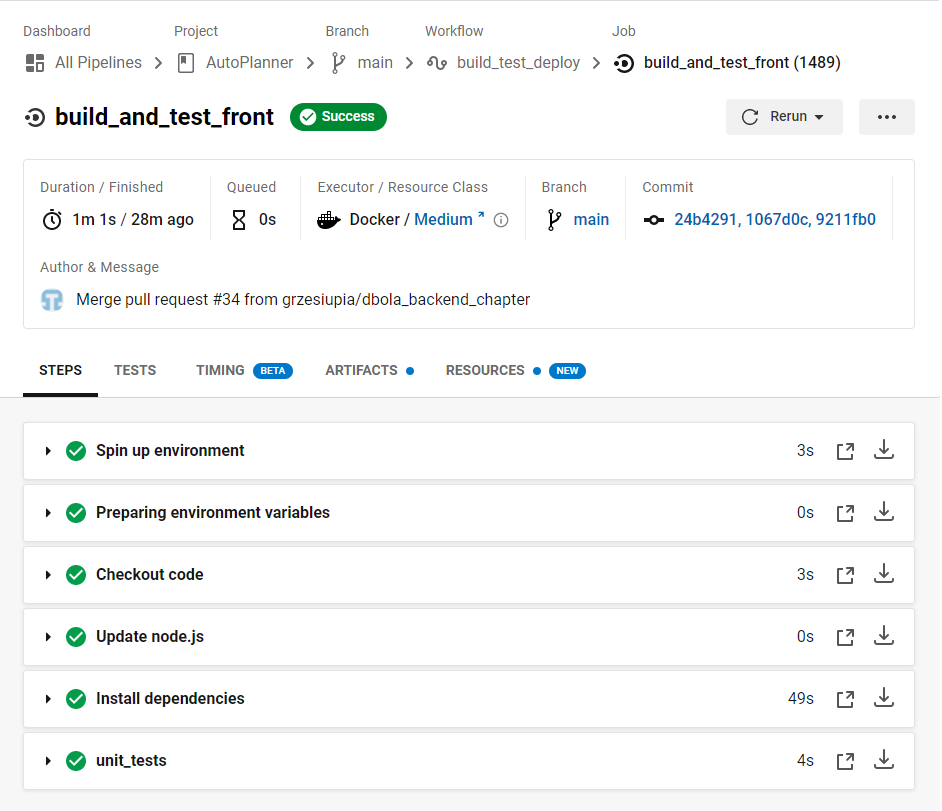
\includegraphics[width=14cm]{figures/circleci_test_front}
\caption{Przykładowy przebieg zadania \textit{build\_and\_text\_front}. Uruchomiony dla zmian wprowadzonych w gałęzi Git \textit{main}.}\label{rys:test_front}
\end{figure}
	
\begin{lstlisting}[caption=Część skryptu config.yml odpowiadająca za wykonanie zadania \textit{deploy\_frontend},label={lst:deploy_front}]
deploy_frontend:
    executor: aws-cli/default
    steps:
      - checkout
      - aws-cli/setup:
          aws-access-key-id: AWS_ACCESS_KEY_ID_FRONT
          aws-secret-access-key: AWS_SECRET_ACCESS_KEY_FRONT
      - run:
          name: deploy_frontend
          command: |
            sudo apt-get update
            # SSH to the server to deploy and Perform steps to deploy
            ssh -o StrictHostKeyChecking=no $EC2_USERNAME@$EC2_PUBLIC_DNS_FRONT 'cd GroupProject; 
            git pull --rebase;
            cd Frontend;
            npm install;
            tmux kill-session -t FRONTEND_SERVER
            sleep 5;
            tmux new-session -d -s "FRONTEND_SERVER";
            tmux send-keys -t FRONTEND_SERVER "npm run serve" C-m;
            exit'
\end{lstlisting}
\newpage
\begin{figure}[H]
\centering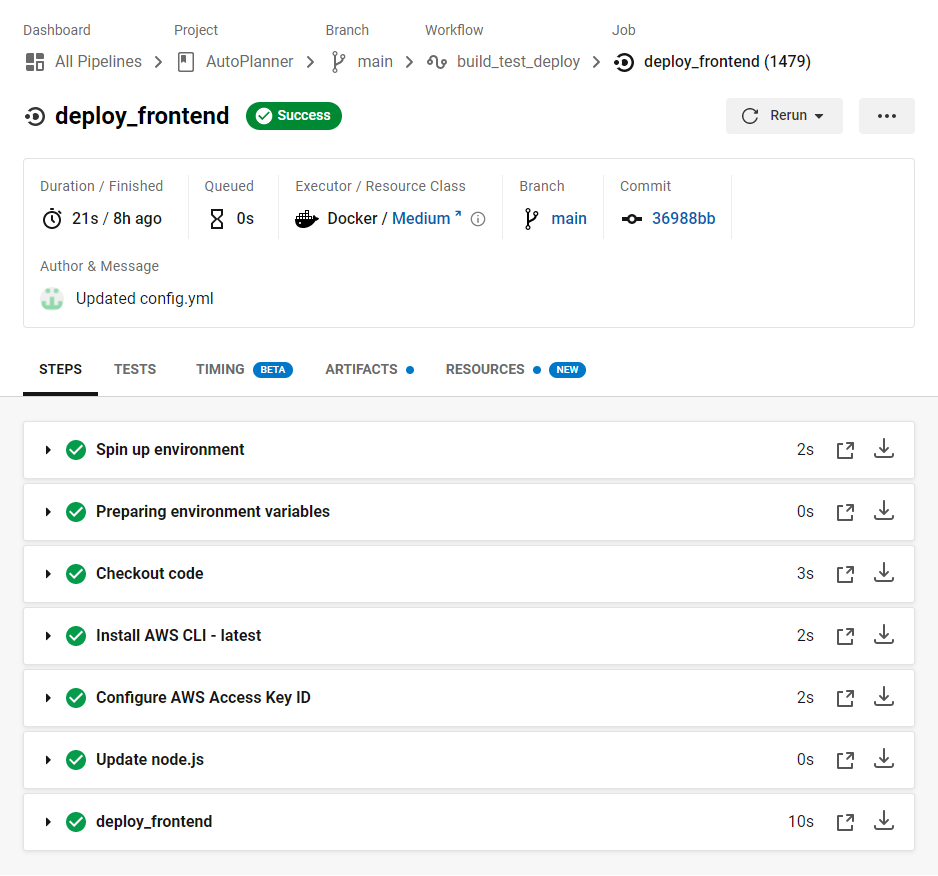
\includegraphics[width=14cm]{figures/circleci_deploy_front}
\caption{Przykładowy przebieg zadania \textit{deploy\_frontend}. Uruchomiony dla zmian wprowadzonych w gałęzi Git \textit{main}.}\label{rys:deploy_front}
\end{figure}


\begin{lstlisting}[caption=Część skryptu config.yml odpowiadająca za wykonanie zadania \textit{deploy\_backend},label={lst:deploy_back}]
deploy_backend:
    executor: aws-cli/default
    steps:
      - checkout
      - aws-cli/setup:
          aws-access-key-id: AWS_ACCESS_KEY_ID_BACK
          aws-secret-access-key: AWS_SECRET_ACCESS_KEY_BACK
      - run:
          name: deploy_back
          command: |
            sudo apt-get update
            # SSH to the server to deploy and Perform steps to deploy
            ssh -o StrictHostKeyChecking=no $EC2_USERNAME@$EC2_PUBLIC_DNS_BACK 'cd GroupProject; 
            git pull --rebase;
            python -m pip install -r requirements.txt;
            cd Backend;
            tmux kill-session -t BACKEND_SERVER
            tmux new-session -d -s "BACKEND_SERVER";
            tmux send-keys -t BACKEND_SERVER "python3 manage.py runserver 0.0.0.0:8000" C-m;
            exit'
\end{lstlisting}
\newpage
\begin{figure}[H]
\centering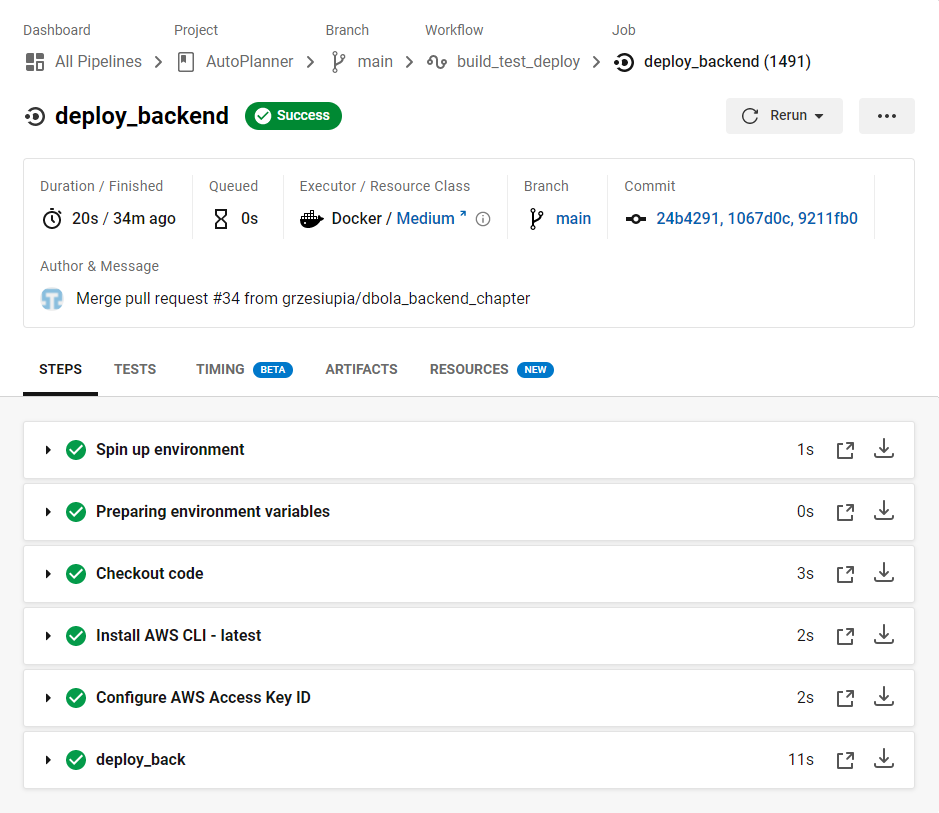
\includegraphics[width=\textwidth]{figures/circleci_deploy_back}
\caption{Przykładowy przebieg zadania \textit{deploy\_backend}. Uruchomiony dla zmian wprowadzonych w gałęzi Git \textit{main}.}\label{rys:deploy_back}
\end{figure}


	\subsection{Zastosowanie DevOps lifecycle od strony GitHub}
	W celu zwiększenia jakości dostarczanych rozwiązań zastosowano następujący przebieg wdrażania. Członek zespołu, chcąc wprowadzić nową funkcjonalność lub rozwinąć już istniejącą, zaciąga najnowszą wersję projektu ze zdalnego repozytorium. Gdy lokalne repozytorium jest zaktualizowane, deweloper tworzy nową gałąź Git, w której będzie wprowadzał zmiany. W momencie gdy autor chce podzielić się swoją pracą z innymi członkami zespołu, publikuje (\textit{push}) swoje zmiany do zdalnego repozytorium oraz tworzy \textit{Pull Request} (PR). W takim PR można prześledzić wszystkie zmiany jakie zostały po kolei wprowadzone przez autora. Każda wprowadzona zmiana pojawiająca się w zdalnym repozytorium wywołuje uruchomienie \textit{pipeline} na platformie CircleCI. Wynik działania zadań z uruchomionego przepływu pracy \textit{pipeline} również można sprawdzić z poziomu PR. W przypadku gdy zmiany wprowadzone w ramach PR przechodzą wszystkie testy oraz nie wywołują żadnych konfliktów, autor prosi o sprawdzenie i zatwierdzenie zmian przez innego członka zespołu. Gdy współpracownik zatwierdzi zmiany, gałąź Git stworzona przez autora na potrzeby zmian może zostać scalona (\textit{merge}) z gałęzią Git \textit{main}. Po wprowadzeniu zmian do gałęxi Git \textit{main} następuje ostatni etap tj. uruchomienie \textit{pipeline} z poziomu tej gałęzi a co za tym idzie, ponowne zbudowanie i przetestowanie aplikacji oraz ostatecznie wdrożenie (zob.~rysunek~\ref{rys:github}).
\begin{figure}[H]
\centering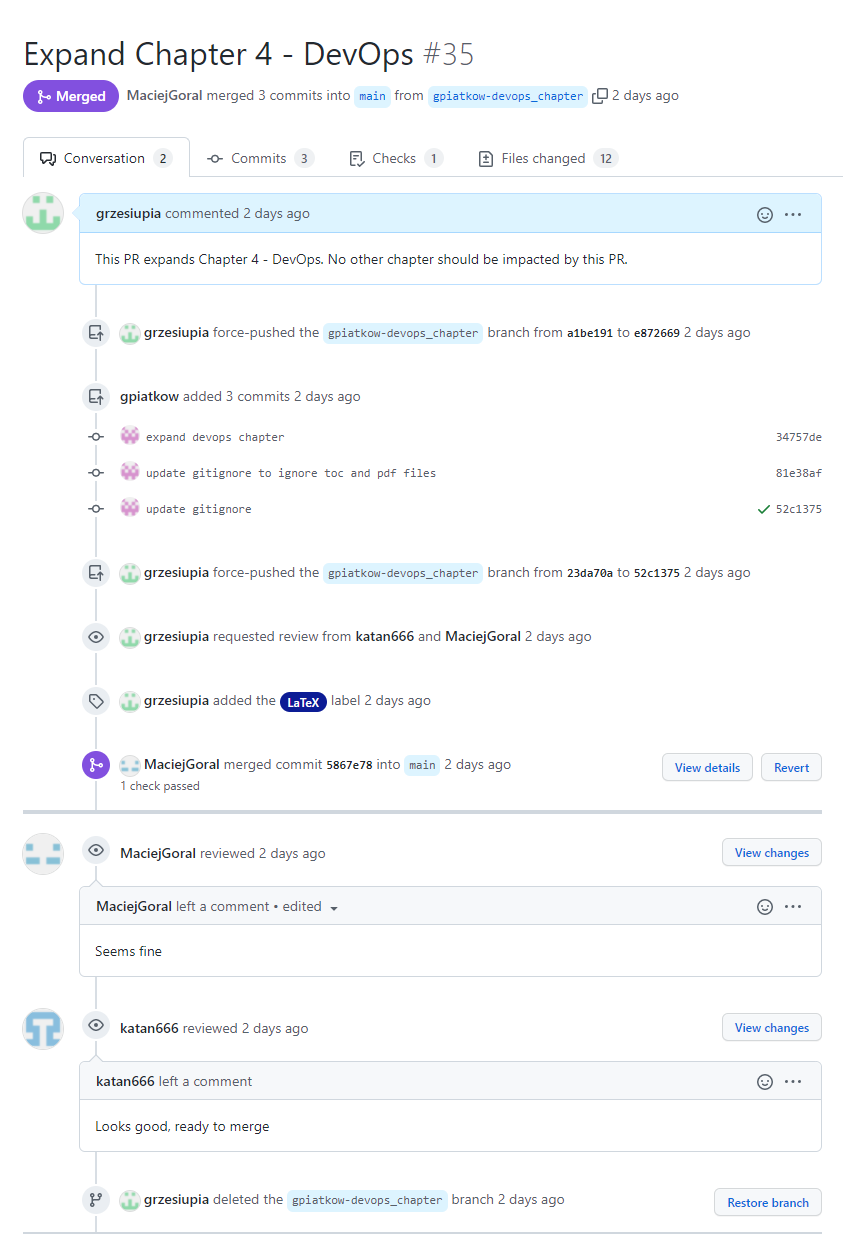
\includegraphics[width=\textwidth]{figures/github_pr}
\caption{Przykładowy przebieg wdrażania zmian przy pomocy \textit{Pull Request}}\label{rys:github}
\end{figure}
	
	 